\documentclass{standalone}
\usepackage{tikz}
\usetikzlibrary{arrows.meta, positioning}
\definecolor{oursCol}{RGB}{34,139,74}
\begin{document}
% Hand-authored (NOT generated by scripts/generate_tikz_figures.py -- that
% script only produces the data-driven figures elsewhere in figures/tikz/).
% Self-contained: no .dat files, no pgfplots.
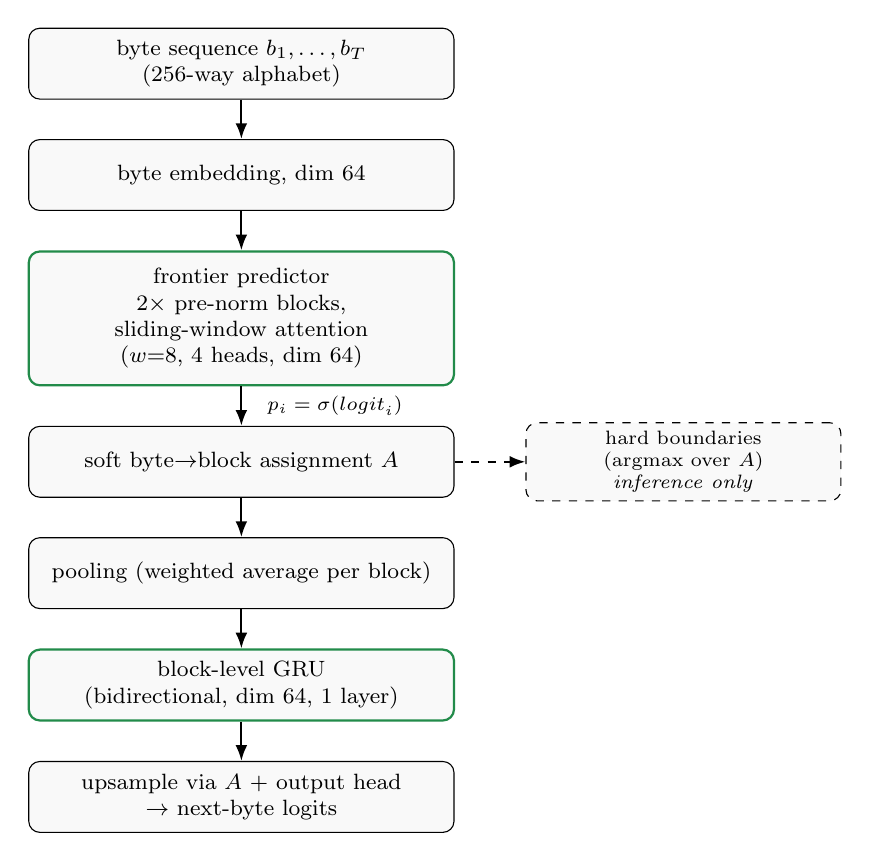
\begin{tikzpicture}[
  node distance=5mm,
  box/.style={draw, rounded corners, align=center, minimum height=9mm,
    minimum width=54mm, font=\footnotesize, inner sep=3pt, fill=gray!5},
  hl/.style={draw=oursCol, line width=0.8pt},
  arr/.style={-{Latex[length=2mm]}, thick},
  lbl/.style={font=\scriptsize, midway, right, align=left, xshift=2mm},
  side/.style={draw, rounded corners, dashed, align=center, minimum height=9mm,
    minimum width=40mm, font=\scriptsize, inner sep=3pt, fill=gray!5}
]
\node[box] (bytes) {byte sequence $b_1,\dots,b_T$\\(256-way alphabet)};
\node[box, below=of bytes] (embed) {byte embedding, dim 64};
\node[box, hl, below=of embed, minimum height=17mm] (frontier)
  {frontier predictor\\2$\times$ pre-norm blocks,\\sliding-window attention\\($w{=}8$, 4 heads, dim 64)};
\node[box, below=of frontier] (assign) {soft byte$\to$block assignment $A$};
\node[box, below=of assign] (pool) {pooling (weighted average per block)};
\node[box, hl, below=of pool] (gru) {block-level GRU\\(bidirectional, dim 64, 1 layer)};
\node[box, below=of gru] (out) {upsample via $A$ + output head\\$\to$ next-byte logits};

\node[side, right=9mm of assign] (hard)
  {hard boundaries\\(argmax over $A$)\\\emph{inference only}};

\draw[arr] (bytes) -- (embed);
\draw[arr] (embed) -- (frontier);
\draw[arr] (frontier) -- node[lbl] {$p_i=\sigma(\text{logit}_i)$} (assign);
\draw[arr] (assign) -- (pool);
\draw[arr] (pool) -- (gru);
\draw[arr] (gru) -- (out);
\draw[arr, dashed] (assign) -- (hard);
\end{tikzpicture}
\end{document}
